\label{part:physics_1}

\textbf{(Implementation Constraints: Boundaries, Media, and Local Mechanisms)}

\bluetext{从抽象状态到可运行系统}

在\ref{part:geometry}中，我们建立了结构、分布、绑定与任务读出的抽象表示。抽象模型若要进入现实任务，还必须回答一组不能由表示空间本身消除的问题：观测从何而来，来源和时序如何验证；状态由什么载体保存和更新，带宽、延迟与故障怎样限制计算；目标怎样变成可执行动作，动作结果又如何反过来修订模型。这里的“实现”不等于把智能还原成某一种材料，也不意味着硬件参数能够直接解释语义与价值。我们关心的是抽象动力学经由哪些接口、资源和局部机制，才成为可测量、可审计、可控制的运行过程。

本篇把这些问题组织为三个相互作用的层次。层次划分依据接口范围和更新时间，而不是宇宙本体的等级。每一层都要声明输入输出类型、状态变量、约束、失败模式和验证方法；跨层关系通过消息、绑定、读出和反馈建立，不以物理名词相似作为机制证明。实际具身系统确有质量、力、温度、功耗和材料老化，这些量在相关章节中按工程单位处理；信息熵、活动强度、目标代价和焦耳能耗则继续保持区分。

本部分将构建一个关于智能体的\textbf{三层实现剖面}模型：
\begin{enumerate}
    \item \textbf{微观层 ($L_{micro}$) — 观测与行动接口}：传感器数据经标定、采样、身份绑定和不确定性估计形成观测事件；目标经资格检查、轨迹细化和局部反馈形成动作。VTE在本书中表示一种可替换的观测编码接口，而不是把现实“量子化”为本体符号的装置。
    \item \textbf{介质层 (The Medium) — 计算与记忆载体}：状态更新依赖处理器、通信链路、存储层和身体结构。我们分析延迟、吞吐、精度、可靠性、实际能耗与老化如何约束可实现的动力学，并区分载体约束、算法复杂度和语义任务难度。
    \item \textbf{宏观层 ($L_{macro}$) — 目标与资源协调}：局部控制、长期目标、风险、授权和资源预算在这里形成可执行的调度状态。系统通过反馈获取信息、消耗资源并维持组织，但耗散结构语言只在真实开放系统条件成立时使用，不能替代目标生成和任务成功的计算说明。
\end{enumerate}

三层之间没有单向决定关系。更快的载体不必然产生更好的任务模型，完善的抽象策略也可能因传感器失准、接口拥塞或执行器饱和而失败。我们将在本篇中分别给出局部估计、有限资源更新、混合状态切换和安全控制的条件，并用故障注入检验跨层闭环。图\ref{fig:trple_mc}保留原有三层视觉结构，但应读作观测接口、运行载体与目标协调之间的计算关系图；其中历史物理术语只提示资源与反馈问题，不构成理论推导。

\begin{figure}[htbp]
    \centering
    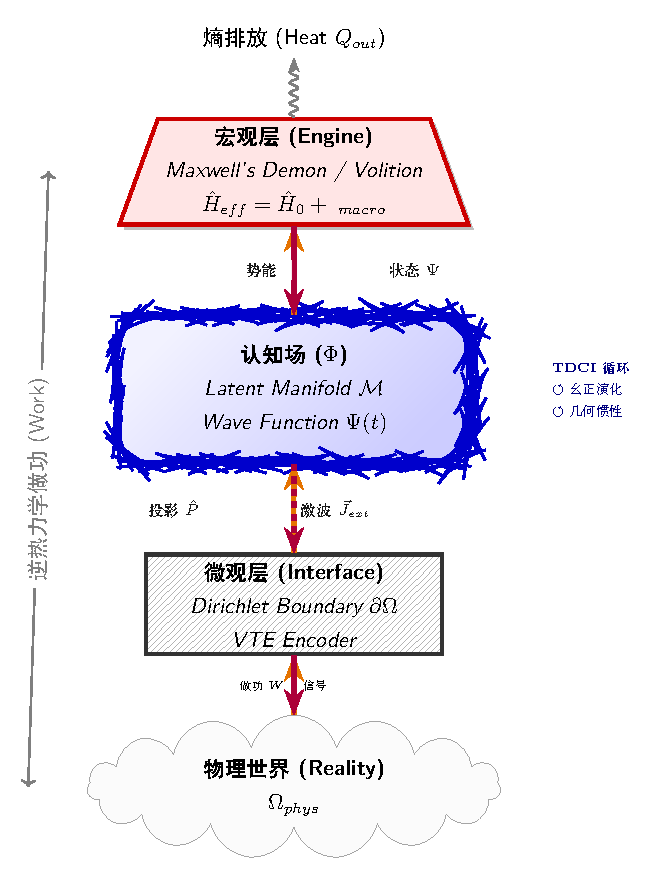
\includegraphics[width=0.96\linewidth,height=0.70\textheight,keepaspectratio]{figure/struct_hsf.pdf}
    \caption{智能系统的三层实现约束：观测接口、运行载体与目标协调}
    \label{fig:trple_mc}
\end{figure}
